\documentclass{beamer}
\usepackage{amsmath, amsthm, amssymb}
\usepackage{enumitem}
\usepackage{tcolorbox}

% Setting up a better font
\usefonttheme{professionalfonts}
\usefonttheme{serif}

\title{Mastermind}
\author{Aaron Berger, Christopher Chute, Matthew Stone}

\begin{document}
    \begin{frame}
    	\maketitle
    \end{frame}

    \begin{frame}
    	\frametitle{Mastermind}
	   	\begin{enumerate}[label=\roman*.]
	    \item Codemaker vs. Codebreaker
	    \item Queries: Guess a vector from $\{1,2,\ldots,6\}^4$
	    \item Response
	    	\begin{enumerate}[label=\roman*.]
			\item Black (Red) hits
			\item White hits
			\end{enumerate}
   	    \end{enumerate}
	    \begin{center}
	    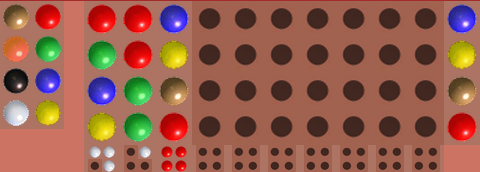
\includegraphics[width=.65\textwidth, keepaspectratio=true]{mm.png}
	    \end{center}
    \end{frame}

    \begin{frame}
    	\frametitle{Knuth Paper -- 1976}
    	\begin{enumerate}[label=\roman*.]
		\item At most five turns needed
		\end{enumerate}
		\begin{tcolorbox}[colback=green!5,colframe=green!40!black,title=Minimax]
		For each possible guess
			\begin{enumerate}[label=]
			\item For each possible response to that guess
				\begin{enumerate}[label=]
				\item Check how many possible solutions remain
				\end{enumerate}
			\item Let \textit{score} be max. number solutions remaining
			\end{enumerate}
		Make guess with minimum score
		\end{tcolorbox}
    \end{frame}
 
    \begin{frame}
    	\frametitle{Extensions}
		\begin{enumerate}[label=\roman*.]
		\item Basic Extension: $n$ spots, $k$ colors
		\item Repeats vs. no repeats
		\item Non-adaptive vs. adaptive strategies
		\end{enumerate}
    \end{frame}
    
    \begin{frame}
    \frametitle{Entropy Method}
    \textit{Surprise Function:} For an event $x$, we want
    	\begin{enumerate}[label=\arabic*.]
		\item $S(x) = 0$ when $\mathbb{P}[x]=1$
		\item $S(x) = 1$ when $\mathbb{P}[x]=1/2$
		\item Decreasing as $\mathbb{P}[x]$ increases\\
		\end{enumerate}
	\begin{enumerate}[label=]
	\item\onslide<2->{Let $S(x)=-\log_2(\mathbb{P}[x])$.}
	\end{enumerate}
	\end{frame}
	
	\begin{frame}
	\frametitle{Entropy Method (cont'd)}
	Entropy is the expected surprise of a random variable.
	\textit{Definition:} Let $X$ be a random variable with domain $D$.
			\begin{equation*}
			H(X) = -\sum_{x\in D}\mathbb{P}[X=x]\cdot\log_2\left(\mathbb{P}[X=x]\right)
			\end{equation*}
%	Key Properties:
%    	\begin{enumerate}[label=\roman*.]
%		\item If random variables $X,Y$ uniquely determine each other's outcomes,
%		then $H(X)=H(Y)$.
%		\item \textit{Subadditivity:} A vector $X=(X_1, X_2, \ldots, X_n)$ of random
%		variables has
%			\begin{equation*}
%			H(X)\le \sum_{i=1}^{n}H(X_i)
%			\end{equation*}
%		\end{enumerate}
%	Use these properties to give lower bound on non-adaptive strategies.
    \end{frame}
    
    \begin{frame}
    \frametitle{Probabilistic Method}
    Non-Adaptive Game: Set of queries $Q=\{q_1, q_2, \ldots, q_s\}$.
    	\begin{align*}
		\mathbb{P}[Q\text{ is a win} & \text{ning set of guesses }] > 0 \\
		& \Downarrow \\
		\exists \text{ a winning } & \text{set of $s$ guesses}
		\end{align*}
    \end{frame}

    \begin{frame}
    \frametitle{Known Bounds}
	\begin{enumerate}[label=\arabic*.]
	\item Lower Bounds: Try to beat $O(n)$.
	\item Upper Bounds: Try to achieve/beat $O(n \log k)$
	\end{enumerate}
    \end{frame}
        
    \begin{frame}
    \frametitle{Bucket Method}
   		\begin{center}
		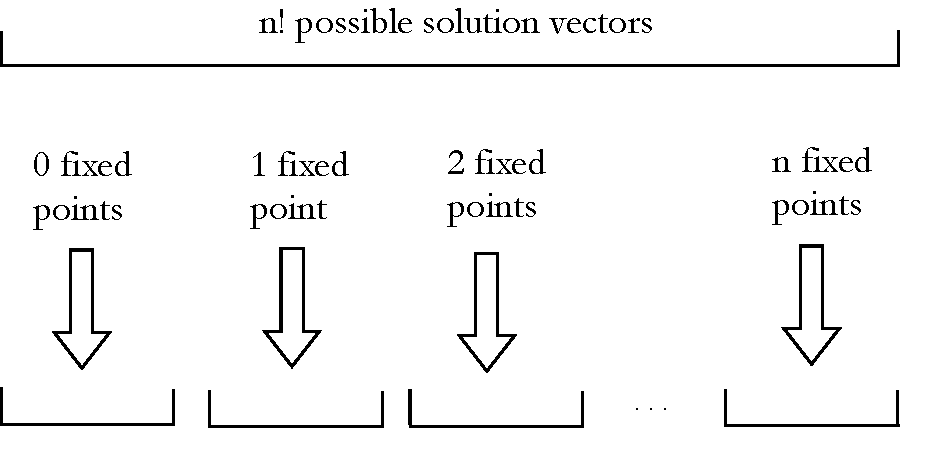
\includegraphics[keepaspectratio=true, width=0.6\textwidth]{buckets.pdf}
		\end{center}
		\begin{enumerate}[label=\roman*.]
		\item Uses more information than previous proofs, using ``buckets.''
		\item Bucket $i$ $\Leftarrow\Rightarrow$ $i$ fixed points
		\item Size of buckets:
			\begin{align*}
			|B_i| & = \binom{n}{i}\cdot D(n-i)\\
			& = \binom{n}{i} \cdot(n-i)!\cdot\sum_{j=0}^{n-i}\frac{(-1)^j}{j!}
			\end{align*}
		\end{enumerate}
    \end{frame}
    
    \begin{frame}
    \frametitle{Deriving $n\log\log n$ Upper Bound when $k=n$}
    [Doerr et. al., 2013]
    	\begin{enumerate}[label=\roman*.]
		\item Split hidden vector into ``coins'' (subvectors).
		\item Use coin weighing problem to eliminate colors.
		\end{enumerate}
    \end{frame}
    
    \begin{frame}
    \frametitle{Non-Adaptive Strategies}
    	\begin{enumerate}[label=\roman*.]
		\item Random Guessing
		\item Evaluate probability of success
		\end{enumerate}
    \end{frame}
    
    
%    \begin{frame}
%    	\frametitle{Minimax Example}
%		\begin{enumerate}[label=\roman*.]
%		\item Hidden Vector: $(3, 5, 0, 0)$
%		\item What to guess? Eliminate as many as possible.
%		\item Simulation [Format: Number Remaining $\rightarrow$ Guess $\rightarrow$
%		(Black Hits, White Hits)]
%			\begin{align*}
%			1296 & \rightarrow \onslide<2->{(0, 0, 1, 1)\rightarrow}
%			\onslide<3->{(0, 2)}\\
%			\onslide<4->{96}
%			\onslide<5->{& \rightarrow (1, 2, 3, 3) \rightarrow (0, 1)\\
%			14 & \rightarrow (4, 1, 0, 4) \rightarrow (1, 0)\\
%			3 & \rightarrow (2, 5, 0, 0) \rightarrow (3, 0)\\
%			1 & \rightarrow (3, 5, 0, 0) \rightarrow (4, 0)}
%			\end{align*}
%		\end{enumerate}
%    \end{frame}

%    \begin{frame}
%    	\frametitle{Known Bounds}
%		\begin{enumerate}[label=\arabic*.]
%		\item\textit{Mastermind with Repeats:}
%   		\begin{enumerate}[label=\roman*.]
%    		\item When $n\le k \le n^2\log\log(n)$, [Chvatal] and [Doerr, et. al.]
%    			\begin{equation*}
%    			\frac{n\log(k)}{\log\binom{n+2}{2}}\le f(n, k)\le O(n\log\log(n))
%    			\end{equation*}
%    		\item When $k=n^{\alpha}$ for $0<\alpha<1$, [Doerr, et. al.]
%    			\begin{equation*}
%    			f(n, k) = \Theta(n)
%    			\end{equation*}
%    		\end{enumerate}
%		\end{enumerate}
%	\end{frame}
%	\begin{frame}
%	\frametitle{Known Bounds (cont.)}
%		\begin{enumerate}[label=\arabic*.]
%		\setcounter{enumi}{1}
%		  	\item\textit{Mastermind without Repeats:} 
%    		\begin{enumerate}[label=\roman*.]
%    		\item When $n=k$, we have the permutation game:
%			[Our Result] and [Ouali et. al]
%    			\begin{equation*}
%    			n - \log\log(n) \le f(n, k)\le n\log(n) + O(n)
%    			\end{equation*}
%   		\end{enumerate}
%	\end{enumerate}
%    \end{frame}

%    \begin{frame}
%    \frametitle{Are You The One?}
%    	\begin{center}
%		
\includegraphics[width=0.7\textwidth, keepaspectratio=true]{ayto1.jpg}
%		\end{center}
%    	\begin{enumerate}[label=\roman*.]
%		\item Essentially Mastermind with $n=k$ and no repeats.
%		\item But queries are different:
%			\begin{enumerate}[label=\alph*.]
%			\item Truth Booth: Single-spot query.
%			\item Perfect Matching: Permutation query with black hits only.
%			\end{enumerate}
%		\end{enumerate}
%    \end{frame}

%    \begin{frame}
%    \frametitle{Future Topics to Explore}
%    	\begin{enumerate}[label=\roman*.]
%		\item Alternative Queries: Can query any subgraph
%		\item Does our lower bound extend to general $n$ and $k$?
%		\item Non-adaptive strategies: Submit all guesses at beginning
%		\end{enumerate}
%    \end{frame}
\end{document}





























